\documentclass[serif]{beamer}\usepackage[]{graphicx}\usepackage[]{color}
%% maxwidth is the original width if it is less than linewidth
%% otherwise use linewidth (to make sure the graphics do not exceed the margin)
\makeatletter
\def\maxwidth{ %
  \ifdim\Gin@nat@width>\linewidth
    \linewidth
  \else
    \Gin@nat@width
  \fi
}
\makeatother

\definecolor{fgcolor}{rgb}{0.345, 0.345, 0.345}
\newcommand{\hlnum}[1]{\textcolor[rgb]{0.686,0.059,0.569}{#1}}%
\newcommand{\hlstr}[1]{\textcolor[rgb]{0.192,0.494,0.8}{#1}}%
\newcommand{\hlcom}[1]{\textcolor[rgb]{0.678,0.584,0.686}{\textit{#1}}}%
\newcommand{\hlopt}[1]{\textcolor[rgb]{0,0,0}{#1}}%
\newcommand{\hlstd}[1]{\textcolor[rgb]{0.345,0.345,0.345}{#1}}%
\newcommand{\hlkwa}[1]{\textcolor[rgb]{0.161,0.373,0.58}{\textbf{#1}}}%
\newcommand{\hlkwb}[1]{\textcolor[rgb]{0.69,0.353,0.396}{#1}}%
\newcommand{\hlkwc}[1]{\textcolor[rgb]{0.333,0.667,0.333}{#1}}%
\newcommand{\hlkwd}[1]{\textcolor[rgb]{0.737,0.353,0.396}{\textbf{#1}}}%

\usepackage{framed}
\makeatletter
\newenvironment{kframe}{%
 \def\at@end@of@kframe{}%
 \ifinner\ifhmode%
  \def\at@end@of@kframe{\end{minipage}}%
  \begin{minipage}{\columnwidth}%
 \fi\fi%
 \def\FrameCommand##1{\hskip\@totalleftmargin \hskip-\fboxsep
 \colorbox{shadecolor}{##1}\hskip-\fboxsep
     % There is no \\@totalrightmargin, so:
     \hskip-\linewidth \hskip-\@totalleftmargin \hskip\columnwidth}%
 \MakeFramed {\advance\hsize-\width
   \@totalleftmargin\z@ \linewidth\hsize
   \@setminipage}}%
 {\par\unskip\endMakeFramed%
 \at@end@of@kframe}
\makeatother

\definecolor{shadecolor}{rgb}{.97, .97, .97}
\definecolor{messagecolor}{rgb}{0, 0, 0}
\definecolor{warningcolor}{rgb}{1, 0, 1}
\definecolor{errorcolor}{rgb}{1, 0, 0}
\newenvironment{knitrout}{}{} % an empty environment to be redefined in TeX

\usepackage{alltt}
\usetheme{Boadilla}
\usepackage{graphicx}
\usepackage[final]{animate}
\usepackage{breqn}
\usepackage{xcolor}
\usepackage{booktabs}
\usepackage{tikz}
\usetikzlibrary{decorations.pathreplacing}
\usetikzlibrary{shapes,arrows,positioning,shadows}
\usepackage{subfig}
\usepackage{pgf}

% change format of enumerated lists
\setbeamertemplate{enumerate items}[default]

\setbeamertemplate{navigation symbols}{}

%tikz objects
\tikzstyle{decision} = [diamond, draw, text width=6em, text badly centered, inner sep=2pt, top color=white, bottom color=zissou3]
\tikzstyle{block} = [rectangle, draw, text width=10em, text centered, rounded corners, minimum height=3em, minimum width=8em, top color = white, bottom color=zissou3]
\tikzstyle{declare} = [rectangle, draw, text width=10em, text centered, minimum height=3em, minimum width=8em, top color = white, bottom color=zissou3]

% knitr setup


% dependent data


% custom colors
\definecolor{zissou1}{HTML}{3B9AB2}\definecolor{zissou2}{HTML}{78B7C5}\definecolor{zissou3}{HTML}{EBCC2A}\definecolor{zissou4}{HTML}{E1AF00}\definecolor{zissou5}{HTML}{F21A00}

% my custom ggplot theme


% figure used on title page


\setbeamercolor{title}{fg=zissou1} % main title
\setbeamercolor{frametitle}{fg=zissou3, bg=zissou2} % frame titles
\setbeamercolor{structure}{fg=zissou5} % bottom banner
\setbeamercolor{normal text}{fg=zissou1}
\usebackgroundtemplate{
\includegraphics[height=\paperheight,width=\paperwidth]{fig/back_tmp.pdf}}
\IfFileExists{upquote.sty}{\usepackage{upquote}}{}
\begin{document}

\title[Evaluating water quality]{\textbf{The search for truth in numbers: Quantitative approaches for evaluating trends in water quality data}}
\author[M. Beck]{Marcus W. Beck}

\institute[USEPA]{ORISE post-doc, USEPA National Health and Environmental Effects Research Laboratory, Gulf Ecology Division, \href{mailto:beck.marcus@epa.gov}{beck.marcus@epa.gov}, Phone: 8509342480}

\date{Oct. 24, 2014}

\titlegraphic{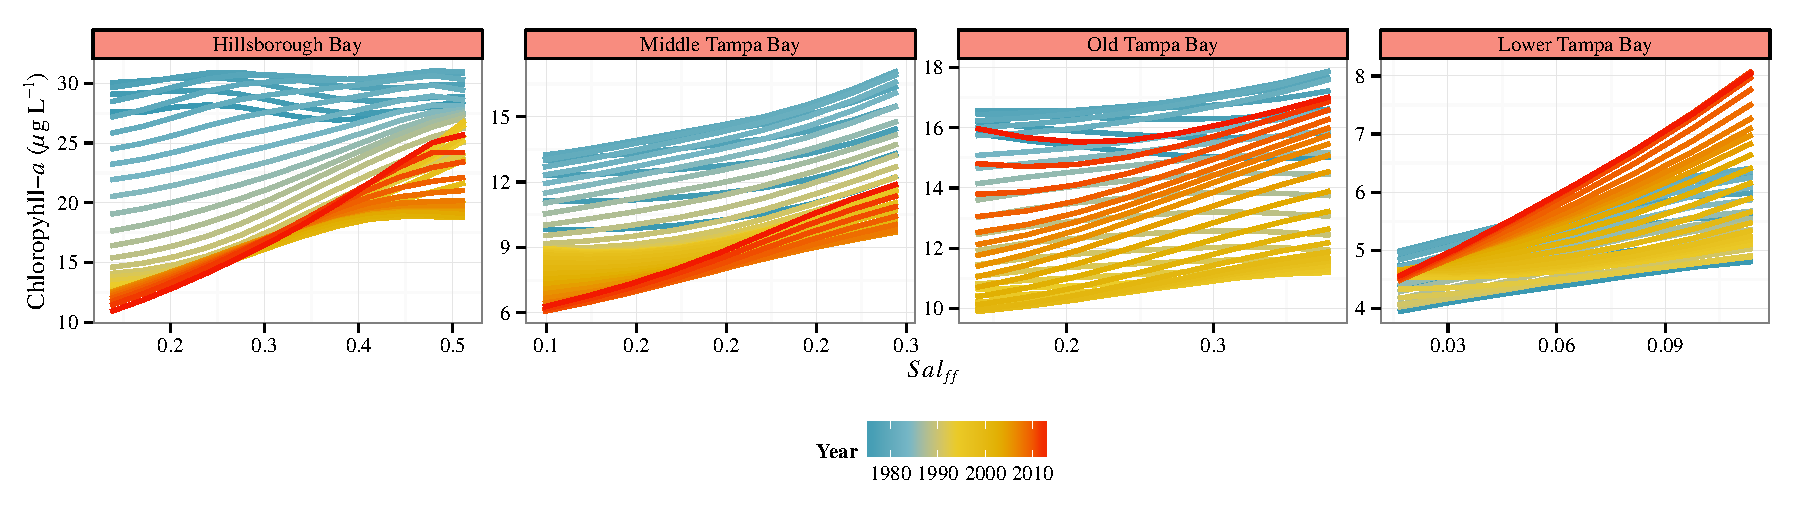
\includegraphics[width=0.95\linewidth]{fig/title_plo.pdf}}

%%%%%%
\begin{frame}[shrink]
\titlepage
\end{frame}

\section{Background}

%%%%%%
\begin{frame}{\textbf{The eutrophication paradigm}}{\textbf{Research and management in coastal waters}}
\onslide<+->
\begin{quote}
Eutrophication (noun) - an \alert{increase} in the rate of supply of \alert{organic matter} to an ecosystem\\~\\
\vspace{0.05in}
\hfill -- \cite{Nixon95}
\end{quote}
\begin{center}
\scalebox{1}{
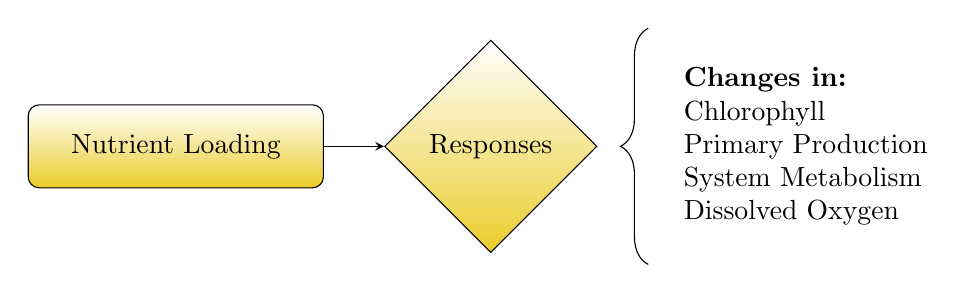
\begin{tikzpicture}[node distance = 4cm, auto, >=stealth]
  \onslide<+->{
  \node[block] (a) {Nutrient Loading};}
  \onslide<+->{
	\node[decision] (b)  [right of=a] {Responses};
 	\draw[->] (a) -- (b);}
  \onslide<+->{
  \draw[decorate,decoration={brace,amplitude=10pt}] [right of=b] (2,-1.5) -- (2,1.5);
  \node[draw,align=left,draw=none] [right of=b] {\textbf{Changes in:}\\ Chlorophyll\\ Primary Production\\ System Metabolism\\ Dissolved Oxygen};}
\end{tikzpicture}}
\end{center}
\vspace{-0.5cm}\hspace*{15pt}\scalebox{0.7}{\hbox{\tiny Adapted from \cite{Cloern01}}}\\~\\
\end{frame}

%%%%%%
\begin{frame}{\textbf{The eutrophication paradigm}}{\textbf{Research and management in coastal waters}}
\onslide<+->
Human inputs can greatly accelarate eutrophication... particularly for coastal waters \\~\\
\begin{itemize}
\onslide<+->
\item Depletion of bottom water dissolved oxygen \cite{Diaz08}
\onslide<+->
\item Increase in frequency/severity of harmful algal blooms \cite{Glibert13}
\onslide<+->
\item Reduction or extirpation of seagrass communities \cite{Tomasko05}
\onslide<+->
\item Propogated effects to upper trophic levels \cite{Powers05}
\end{itemize}
\end{frame}

%%%%%%
\begin{frame}{\textbf{The eutrophication paradigm}}{\textbf{Research and management in coastal waters}}
\centerline{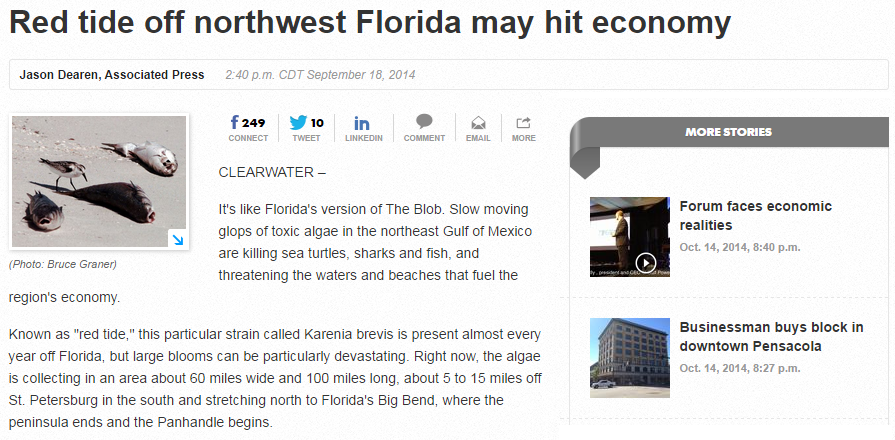
\includegraphics[width = 0.95\textwidth]{fig/redtide.png}}
\end{frame}

%%%%%%
\begin{frame}{\textbf{The eutrophication paradigm}}{\textbf{Research and management in coastal waters}}
\onslide<+->
Water Quality Act Amendments of 1972 \\~\\
\begin{itemize}
\item Federal mandates to \alert{protect and restore} the chemical, physical, and biological integrity of \alert{surface waters}
\item Protection and restoration requires \alert{criteria} \\~\\
\end{itemize}
\onslide<+->
Numeric nutrient criteria \\~\\
\begin{itemize}
\item The amounts of contaminants or pollutants that may be present without impairing aquatic life or human health 
\item E.g., nutrients limits for seagrass in Indian River Lagoon...
\end{itemize}
\end{frame}

%%%%%%
\begin{frame}{\textbf{The eutrophication paradigm}}{\textbf{Research and management in coastal waters}}
\onslide<+->
Nutrient limits using seagrass depth-limit targets \tiny \cite{Steward07}\\~\\
\begin{columns}[T]
\begin{column}{0.45\textwidth}
\centerline{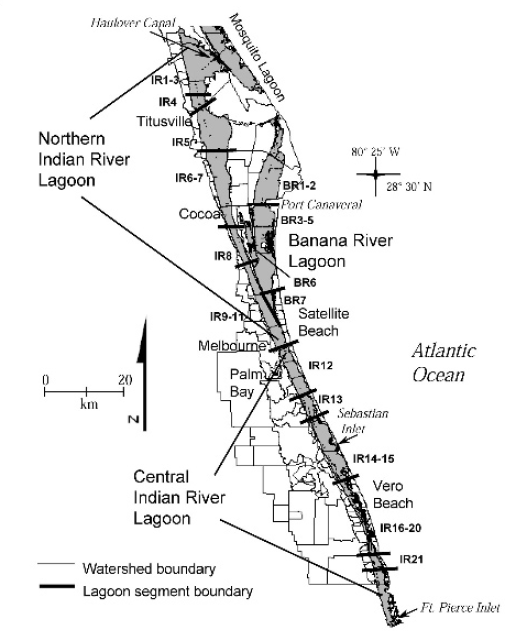
\includegraphics[width = 0.9\textwidth]{fig/irl_map.png}}
\end{column}
\begin{column}{0.45\textwidth}
\centerline{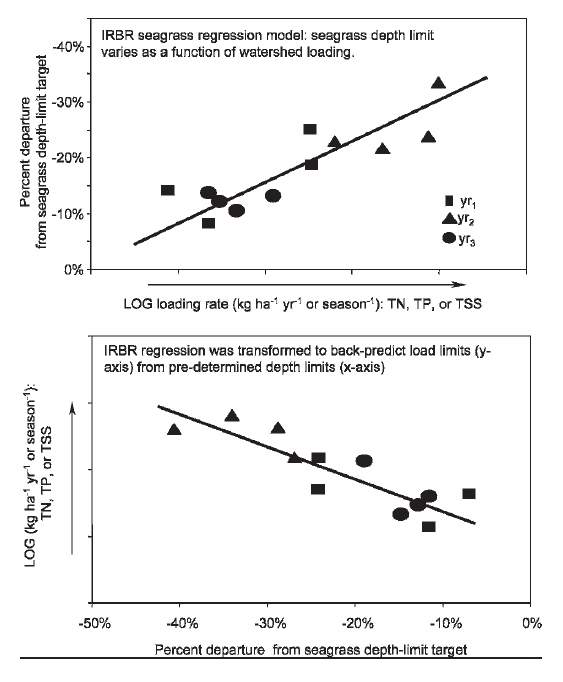
\includegraphics[width = 0.92\textwidth]{fig/irl_reg.png}}
\end{column}
\end{columns}
\end{frame}

%%%%%%
\begin{frame}{\textbf{The eutrophication paradigm}}{\textbf{Research and management in coastal waters}}
\onslide<+->
USEPA national strategy for the development of regional nutrient criteria\\~\\
\begin{itemize}
\item Aid states' ability to control and reduce nutrient enrichments \\~\\
\item Responsibility of EPA to develop criteria guidance \\~\\
\end{itemize}
\scriptsize
\hfill \cite{USEPA98}
\end{frame}

%%%%%%
\begin{frame}{\textbf{The eutrophication paradigm}}{\textbf{Research and management in coastal waters}}
USEPA Gulf Ecology Division - guidance to Florida DEP and others on criteria development for estuaries \\~\\
\centerline{\includegraphics[width = 0.8\textwidth]{fig/sabine.png}}
\end{frame}

%%%%%%
\begin{frame}{\textbf{The eutrophication paradigm}}{\textbf{Challenges for criteria development}}
\onslide<+->
There are challenges to providing guidance...\\~\\
\alert{Challenge 1:} We don't fully understand eutrophication processes \\~\\
\begin{quote}
There are good reasons to believe that eutrophication will, in the near \alert{future}, become a \alert{hazard in marine coastal areas} in many parts of the world.\\~\\
\vspace{0.05in}
\hfill -- \cite{Rosenberg85} \\~\\
\end{quote}
\end{frame}

%%%%%
\begin{frame}{\textbf{The eutrophication paradigm}}{\textbf{Challenges for criteria development}}
\onslide<+->
Our conceptual model for understanding the effects of nutrient pollution is adopted from freshwater sciences. \\~\\
\begin{center}
\scalebox{1}{
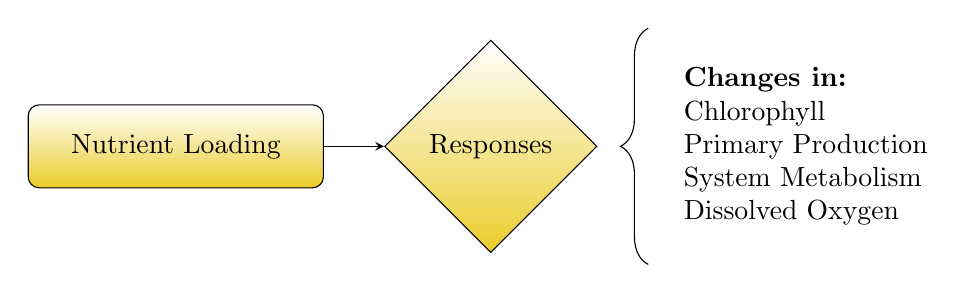
\begin{tikzpicture}[node distance = 4cm, auto, >=stealth]
  \node[block] (a) {Nutrient Loading};
	\node[decision] (b)  [right of=a] {Responses};
 	\draw[->] (a) -- (b);
  \draw[decorate,decoration={brace,amplitude=10pt}] [right of=b] (2,-1.5) -- (2,1.5);
  \node[draw,align=left,draw=none] [right of=b] {\textbf{Changes in:}\\ Chlorophyll\\ Primary Production\\ System Metabolism\\ Dissolved Oxygen};
\end{tikzpicture}}
\end{center}
\vspace{-0.5cm}\hspace*{15pt}\scalebox{0.7}{\hbox{\tiny Adapted from \cite{Cloern01}}}\\~\\
\end{frame}



\begin{frame}{\textbf{The eutrophication paradigm}}{\textbf{Challenges for criteria development}}
Spatial and temporal variation in chlorophyll for Tampa Bay\\~\\
\begin{columns}
\begin{column}{0.53\textwidth}
\begin{center}
\includegraphics<1>[width=\textwidth,trim=0in 0.2in 0.6in 0in]{fig/ggchl_1.pdf}
\includegraphics<2>[width=\textwidth,trim=0in 0.2in 0.6in 0in]{fig/ggchl_2.pdf}
\includegraphics<3>[width=\textwidth,trim=0in 0.2in 0.6in 0in]{fig/ggchl_3.pdf}
\includegraphics<4>[width=\textwidth,trim=0in 0.2in 0.6in 0in]{fig/ggchl_4.pdf}
\includegraphics<5>[width=\textwidth,trim=0in 0.2in 0.6in 0in]{fig/ggchl_5.pdf}
\end{center}
\end{column}
\begin{column}{0.43\textwidth}
\begin{center}
\includegraphics<1>[width=\textwidth]{fig/wbid_map_1.pdf}
\includegraphics<2>[width=\textwidth]{fig/wbid_map_2.pdf}
\includegraphics<3>[width=\textwidth]{fig/wbid_map_3.pdf}
\includegraphics<4>[width=\textwidth]{fig/wbid_map_4.pdf}
\includegraphics<5>[width=\textwidth]{fig/wbid_map_5.pdf}
\end{center}
\end{column}
\end{columns}
\end{frame}

% %%%%%%
% \begin{frame}
% Lots of covariance between parameters that confuses identification of drivers
% tide v do
% salinity v chl
% \end{frame}

%%%%%%
\begin{frame}{\textbf{The eutrophication paradigm}}{\textbf{Challenges for criteria development}}
\onslide<+->
\alert{Challenge 2:} We have the data but often lack tools to unambiguously and quantitatively characterize\\~\\
\onslide<+->
\vspace{0.2in}
\begin{quote}
Data without models are chaos, but models without data are fantasy. \\~\\
\vspace{0.05in}
\hspace{0.1in}-- NWQMC 2014 plenary, R. Hirsch via \cite{Nisbet14}
\end{quote}
\end{frame}

%%%%%%
\begin{frame}[shrink]{\textbf{The eutrophication paradigm}}{\textbf{Challenges for criteria development}}
System Wide Monitoring Program, initiated in 1995 to provide continuous data at over 300 stations in 28 US estuaries \\~\\
\centerline{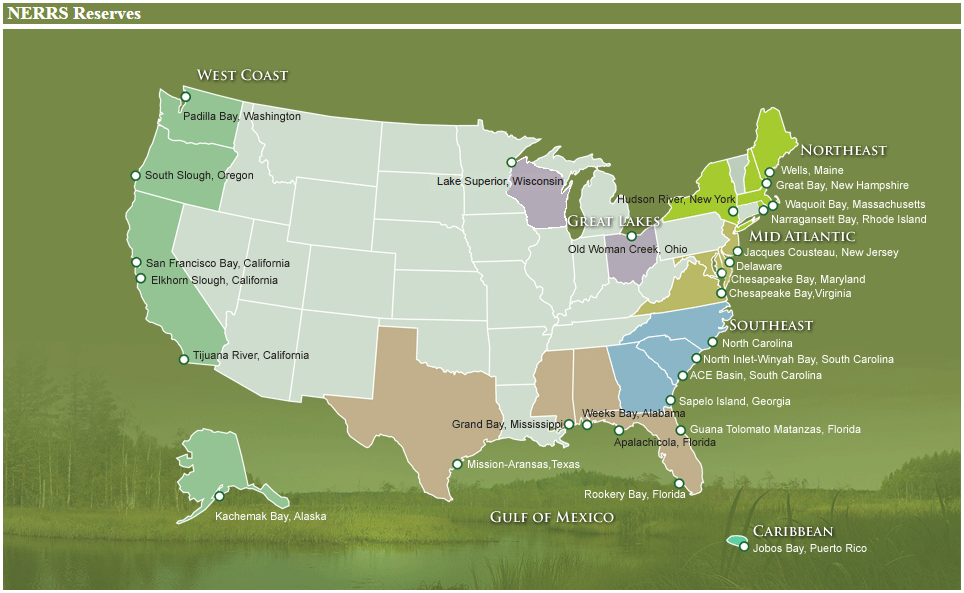
\includegraphics[width = 0.8\textwidth]{fig/NERRS_locations.png}}
\tiny
\flushright
\href{http://nerrs.noaa.gov/ReservesMap.aspx}{http://nerrs.noaa.gov/ReservesMap.aspx}
\end{frame}

%%%%%%
\begin{frame}{\textbf{The eutrophication paradigm}}{\textbf{Challenges for criteria development}}
\onslide<+->
SWMP - As of this month, over 56 million records\\~\\
\begin{itemize}
\item Weather $>$ 13 million
\item Water quality $>$ 43 million
\item Nutrients $>$ 93 thousand \\~\\
\end{itemize}
\onslide<+->
Despite the quantity and quality of the data, very few comparative analyses. Exceptions... \\~\\
\begin{itemize}
\item Comparison of net metabolism \cite{Caffrey03}, \cite{Caffrey04}
\item DO variation between estuaries \cite{Wenner04}
\item Synthesis reports \cite{Wenner01}, \cite{Sanger02}
\end{itemize}
\end{frame}

%%%%%%
\begin{frame}{\textbf{The eutrophication paradigm}}{\textbf{Challenges for criteria development}}
\onslide<+->
Guidance may come in many forms - not just a number \\~\\
\onslide<+->
\alert{Case 1:} Chlorophyll drivers in Tampa Bay\\~\\
\onslide<+->
\alert{Case 2:} Improving our understanding of seagrass growth and water quality\\~\\
\onslide<+->
\alert{Case 3:} `Open-science' tools for analysis of water quality\\~\\
\onslide<+->
Each provides an example of addressing the dual challenges of \alert{understanding nutrient dynamics} and \alert{developing quantitative tools} for trend evaluation 
\end{frame}

\section{Case 1: Tampa Bay}

% tampa bay map, w/ inset


%%%%%%
\begin{frame}{\textbf{Case 1: Tampa Bay}}{\textbf{Understanding chlorophyll response to eutrophication}}
\begin{columns}
\begin{column}{0.5\textwidth}
\begin{itemize}
\item Four bay segments\\~\\
\item Monthly wq data at 50 stations from 1974 to present \\~\\
\item Longitudinal profile of nutrient load and salinity \\~\\
\end{itemize}
\vspace{0cm}\hspace*{15pt}\scalebox{0.7}{\hbox{\tiny Data from \cite{TBEP11}}}
\end{column}
\begin{column}{0.5\textwidth}
\centerline{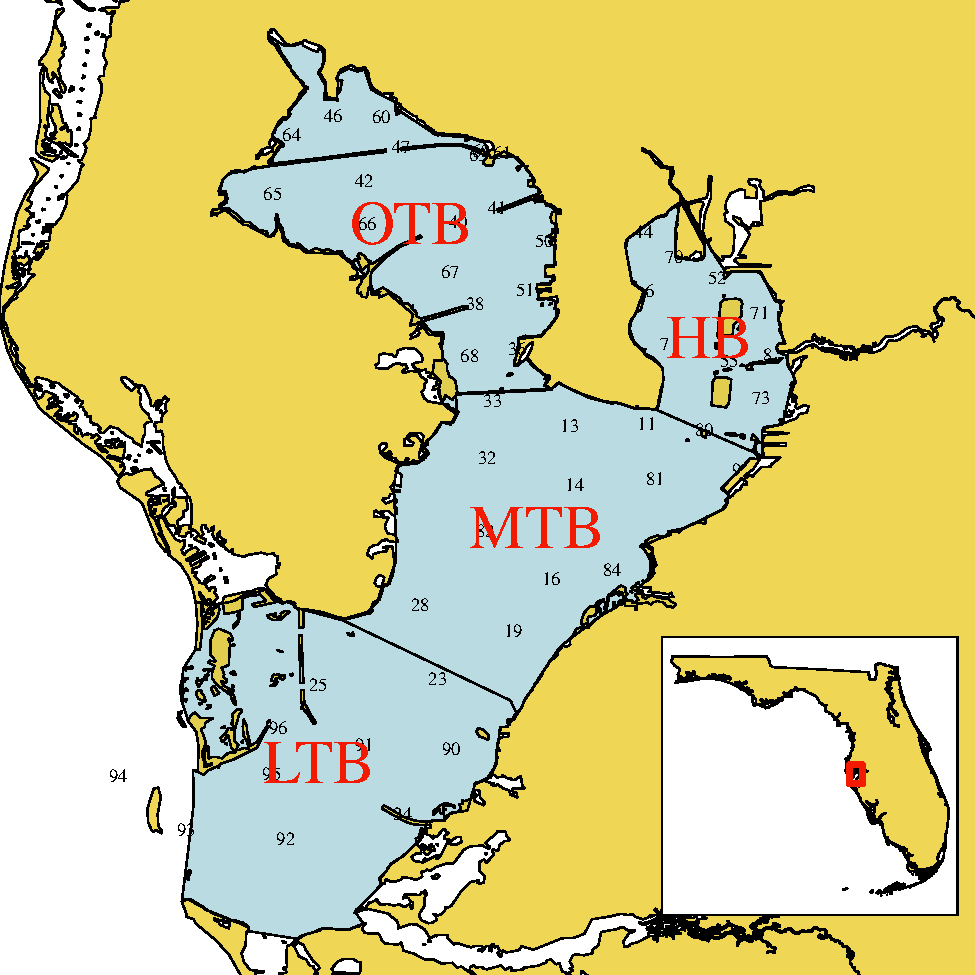
\includegraphics[width = \textwidth]{fig/tb_map.pdf}}
\end{column}
\end{columns}
\end{frame}

%%%%%%
\begin{frame}{\textbf{Case 1: Tampa Bay}}{\textbf{Understanding chlorophyll response to eutrophication}}
\begin{figure}[!ht]


{\centering 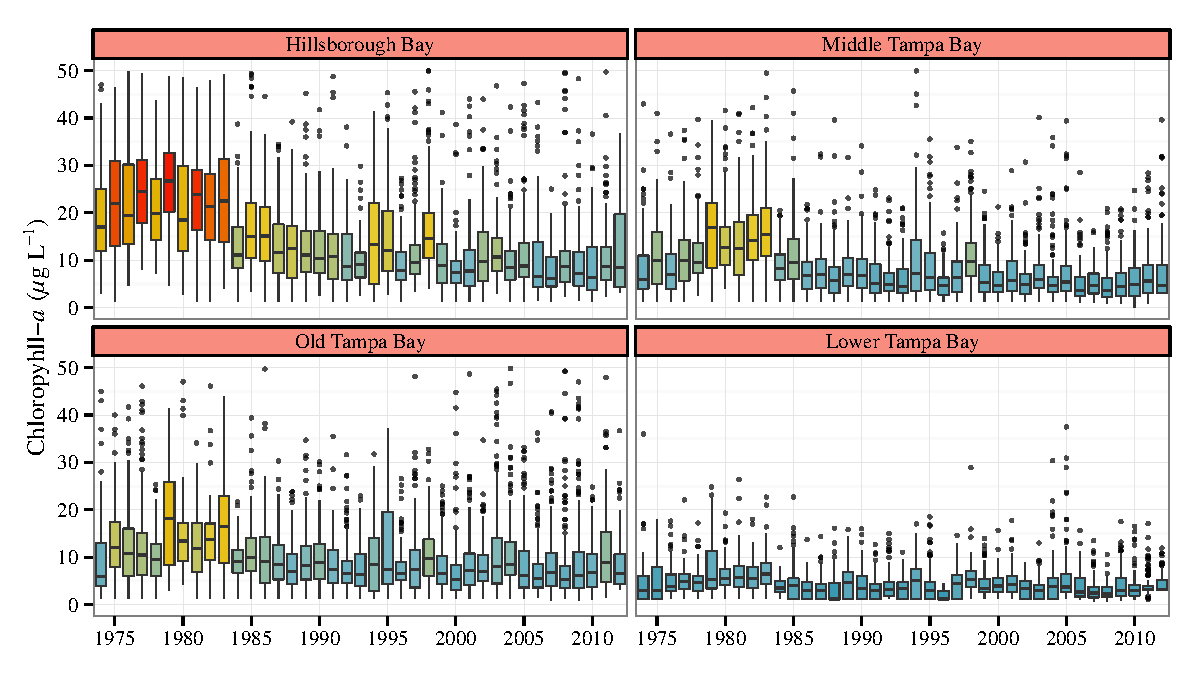
\includegraphics[width=\linewidth]{fig/annual_chl} 

}

\caption[Annual trends in chlorophyll for each bay segment]{Annual trends in chlorophyll for each bay segment.\label{fig:annual_chl}}
\end{figure}


\end{frame}

% variation in chl by year, season, and management

%%%%%%
\begin{frame}{\textbf{Case 1: Tampa Bay}}{\textbf{Understanding chlorophyll response to eutrophication}}
What affects our interpretation of chlorophyll response to nutrients?
\vspace{-0.1in}
\captionsetup[subfloat]{captionskip=0pt, position=top}
\begin{figure}
\centering
\subfloat[]{
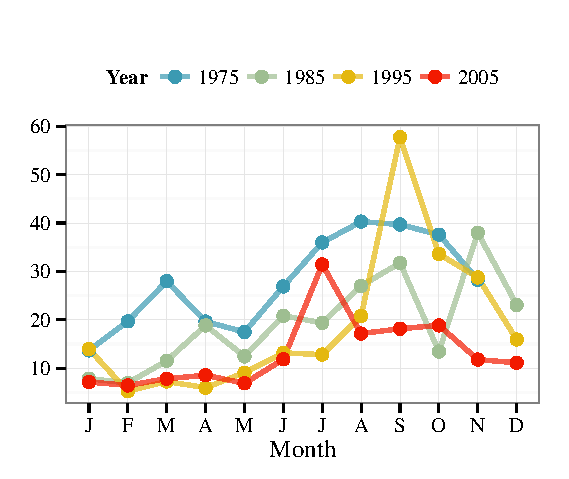
\includegraphics[width=0.46\textwidth,page=1,trim=0.2in 0in 0in 0.35in,clip]{fig/salmoyr.pdf}
\label{fig:salmoyr1}
}
\subfloat[]{
\includegraphics[width=0.46\textwidth,page=2,trim=0.2in 0in 0in 0.35in,clip]{fig/salmoyr.pdf}
\label{fig:salmoyr2}
}

\leavevmode\smash{\makebox[0pt]{\hspace{0em}% HORIZONTAL POSITION           
  \rotatebox[origin=l]{90}{\hspace{3em}% VERTICAL POSITION
    {\color{black} Chlorophyll-\textit{a}}}}}
    \hspace{0pt plus 1filll}\null

\caption{Variation in chlorophyll by {\color{zissou5}\protect\subref{fig:salmoyr1}} time and {\color{zissou5}\protect\subref{fig:salmoyr2}} salinity and management in Hillsborough Bay.  Panel {\color{zissou5}\protect\subref{fig:salmoyr1}} is colored before and after wastewater treatment in 1979.}
\label{fig:salmoyr}
\end{figure}
\captionsetup[subfloat]{position=top}
\end{frame}

%%%%%%
\begin{frame}{\textbf{Case 1: Tampa Bay}}{\textbf{Understanding chlorophyll response to eutrophication}}
\onslide<+->
\begin{block}{Study objective}
Adapt and apply nutrient response model for estuaries that leverages the descriptive capabilities of large datasets
\end{block}
\vspace{0.2in}
\onslide<+->
Questions of management concern -- Can we...
\begin{itemize}
\item ...provide a natural history of water quality that is temporally consistent with drivers of change?
\onslide<+->
\item ...characterize changes in extreme events in addition to describing the mean response?  
\onslide<+->
\item ...improve our understanding of the nutrient-response paradigm in estuaries?
\end{itemize}
\end{frame}

%%%%%%
\begin{frame}{\textbf{Case 1: Tampa Bay}}{\textbf{Understanding chlorophyll response to eutrophication}}
\onslide<+->
The \alert{weighted regression (WRTDS)} model is being developed by USGS for pollutant modelling in rivers \cite{Hirsch10}\\~\\
Based on the idea that pollution concentration is a function of \alert{time}, \alert{discharge}, and \alert{season}\\~\\
\onslide<+->
\alert{Problem:} We want to see if management has an effect on reducing pollutant load over time, but pollutant load varies with discharge.\\~\\
\alert{Solution:} Develop a model that accounts for changes in relationships between drivers of pollution over time.\\~\\
\alert{Adaptation:} Can this approach be used to evaluate chlorophyll trends in Tampa Bay?
\end{frame}



%%%%%%
\begin{frame}{\textbf{Case 1: Tampa Bay}}{\textbf{Understanding chlorophyll response to eutrophication}}
How does weighted regression work?
\begin{center}
\animategraphics[controls,width=\linewidth]{12}{fig/wtex}{}{} %frame rate is 12 per/sec
\end{center}
\end{frame}

%%%%%%
\begin{frame}{\textbf{Case 1: Tampa Bay}}{\textbf{Understanding chlorophyll response to eutrophication}}
This gives us improved predictions of chlorophyll dynamics...
\begin{figure}[!ht]


{\centering 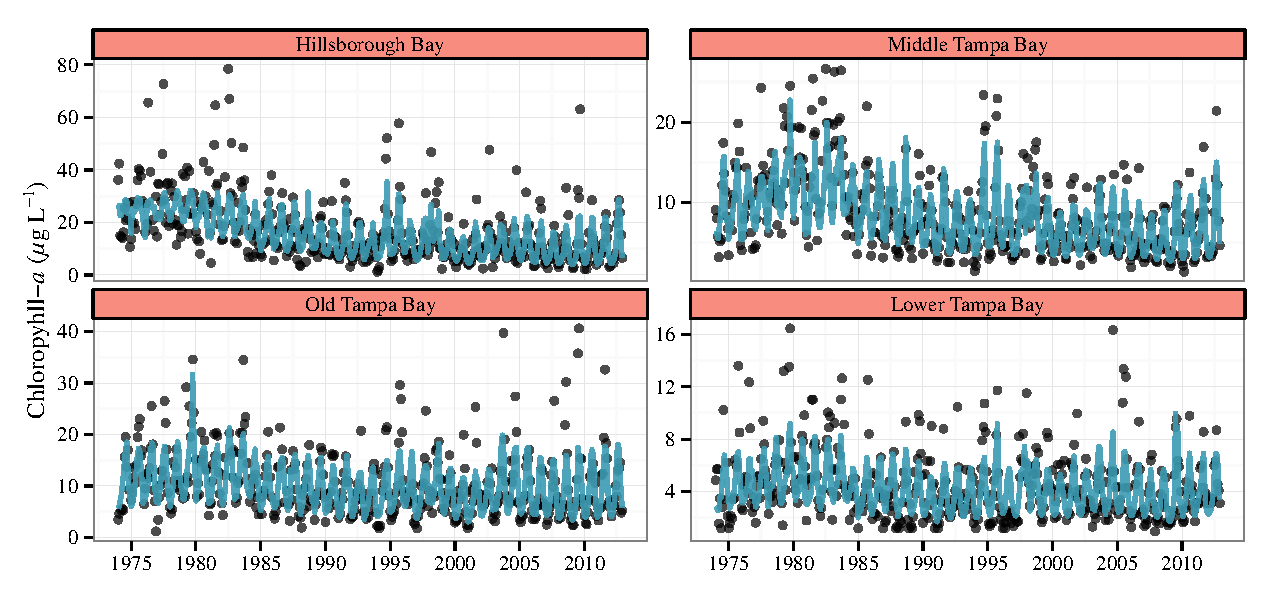
\includegraphics[width=\linewidth]{fig//predvals} 

}

\caption[Predicted and observed monthly chlorophyll by segment]{Predicted and observed monthly chlorophyll by segment.\label{fig:/predvals}}
\end{figure}


\end{frame}



%%%%%%
\begin{frame}{\textbf{Case 1: Tampa Bay}}{\textbf{Understanding chlorophyll response to eutrophication}}
Because the model is dynamic, we have parameters describing the relationship of chlorophyll with other factors specific to different time periods \\~\\
\begin{columns}[T]
\begin{column}{0.45\textwidth}
\centerline{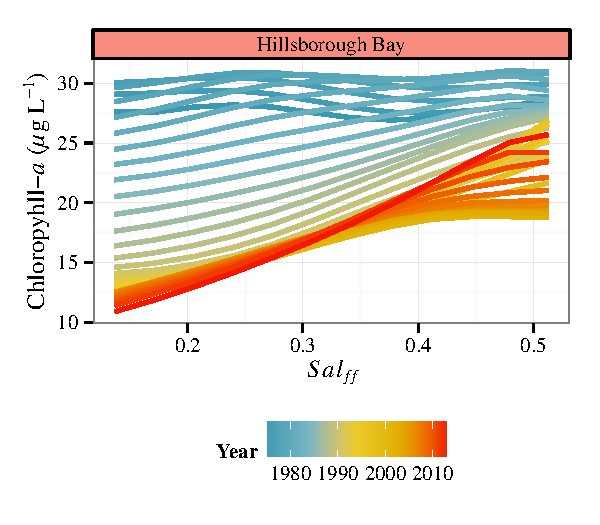
\includegraphics[width = \textwidth]{fig/hill.pdf}}
\end{column}
\begin{column}{0.45\textwidth}
\begin{itemize}
\item Early period (blue) - point-sources
\item Late period (red) - non-point sources
\item Chlorophyll shows increasing response to freshwater input in recent years
\end{itemize}
\end{column}
\end{columns}
\end{frame}

%%%%%%
\begin{frame}{\textbf{Case 1: Tampa Bay}}{\textbf{Understanding chlorophyll response to eutrophication}}
\onslide<+->
What does this mean for Tampa Bay?\\~\\
\begin{itemize}
\item Predictions followed observed chlorophyll -- but increased clarity in the description
\item More detailed evaluation of trends allows greater insight into drivers of change\\~\\
\end{itemize}
\onslide<+->
The model parameters show us a picture...
\centerline{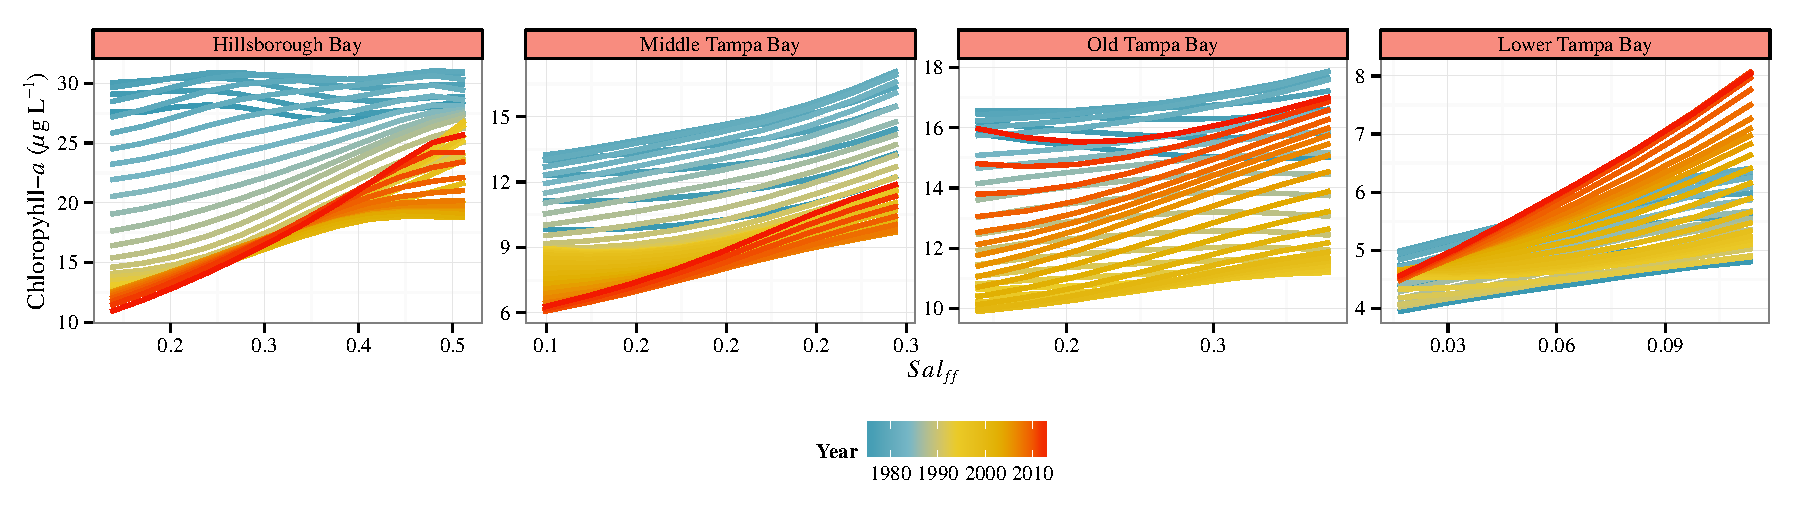
\includegraphics[width = \textwidth]{fig/title_plo.pdf}}
\end{frame}

\section{Case 2: Seagrass and water quality}

%%%%%%
\begin{frame}{\textbf{Case 2: Seagrass and water quality}}{\textbf{Making the most of existing data}}
\begin{center}
Seagrass have long been considered sentinels of water quality \\~\\
\centerline{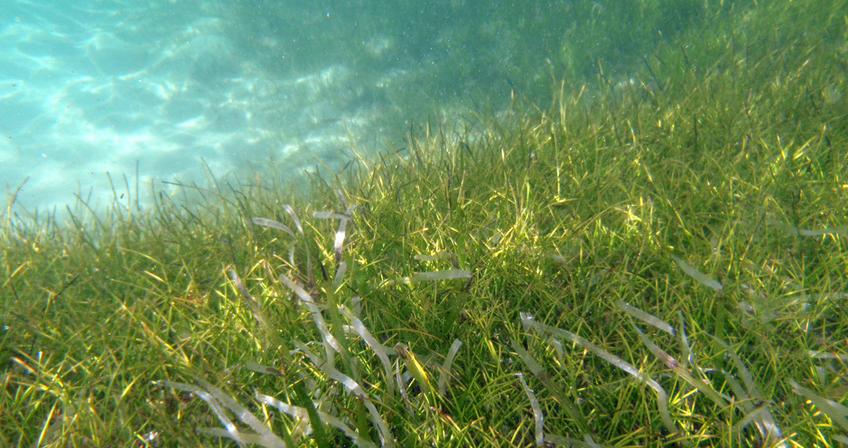
\includegraphics[width = 0.7\textwidth]{fig/sg_pic.png}}
\vspace{0.1in}
Seagrass provide numerous benefits - healthy seagrass, healthy estuary
\end{center}
\vfill
\tiny
\hfill Credit: \href{https://www.flickr.com/photos/swimvixen2/3581613875/in/photostream/}{flickr.com/photos/swimvixen2}
\end{frame}

%%%%%%
\begin{frame}{\textbf{Case 2: Seagrass and water quality}}{\textbf{Making the most of existing data}}
\onslide<+->
The maximum depth of colonization is a useful proxy for trophic state \\~\\
Often used as a basis for establishing nutrient criteria \\~\\
\onslide<+->
\alert{Problem 1:} No consensus on the best way to measure depth of colonization\\~\\
\alert{Problem 2:} Plenty of data are available but standardized techniques have not been developed
\end{frame}

%%%%%%
\begin{frame}{\textbf{Case 2: Seagrass and water quality}}{\textbf{Making the most of existing data}}
\onslide<+->
\alert{Solution 1:} Develop a reproducible and empirical method for estimating depth of colonization \scriptsize [Hagy et al., in prep]
\begin{columns}[T]
\begin{column}{0.5\textwidth}
\begin{knitrout}
\definecolor{shadecolor}{rgb}{0.969, 0.969, 0.969}\color{fgcolor}

{\centering 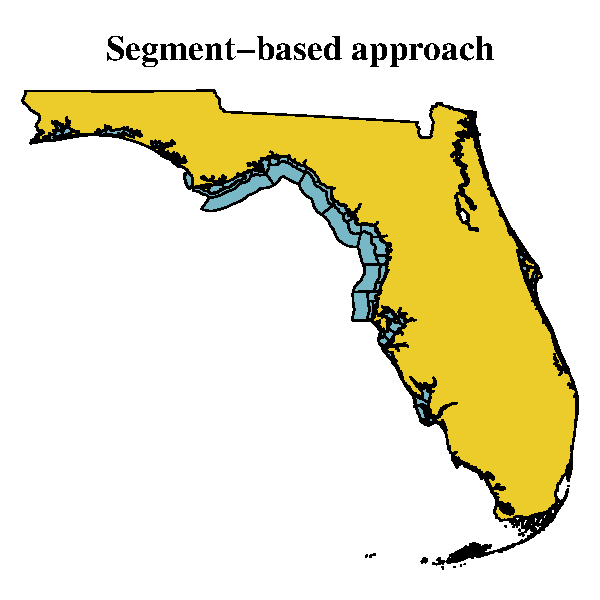
\includegraphics[width=\maxwidth]{fig//segmap} 

}



\end{knitrout}
\end{column}
\begin{column}{0.45\textwidth}
\centerline{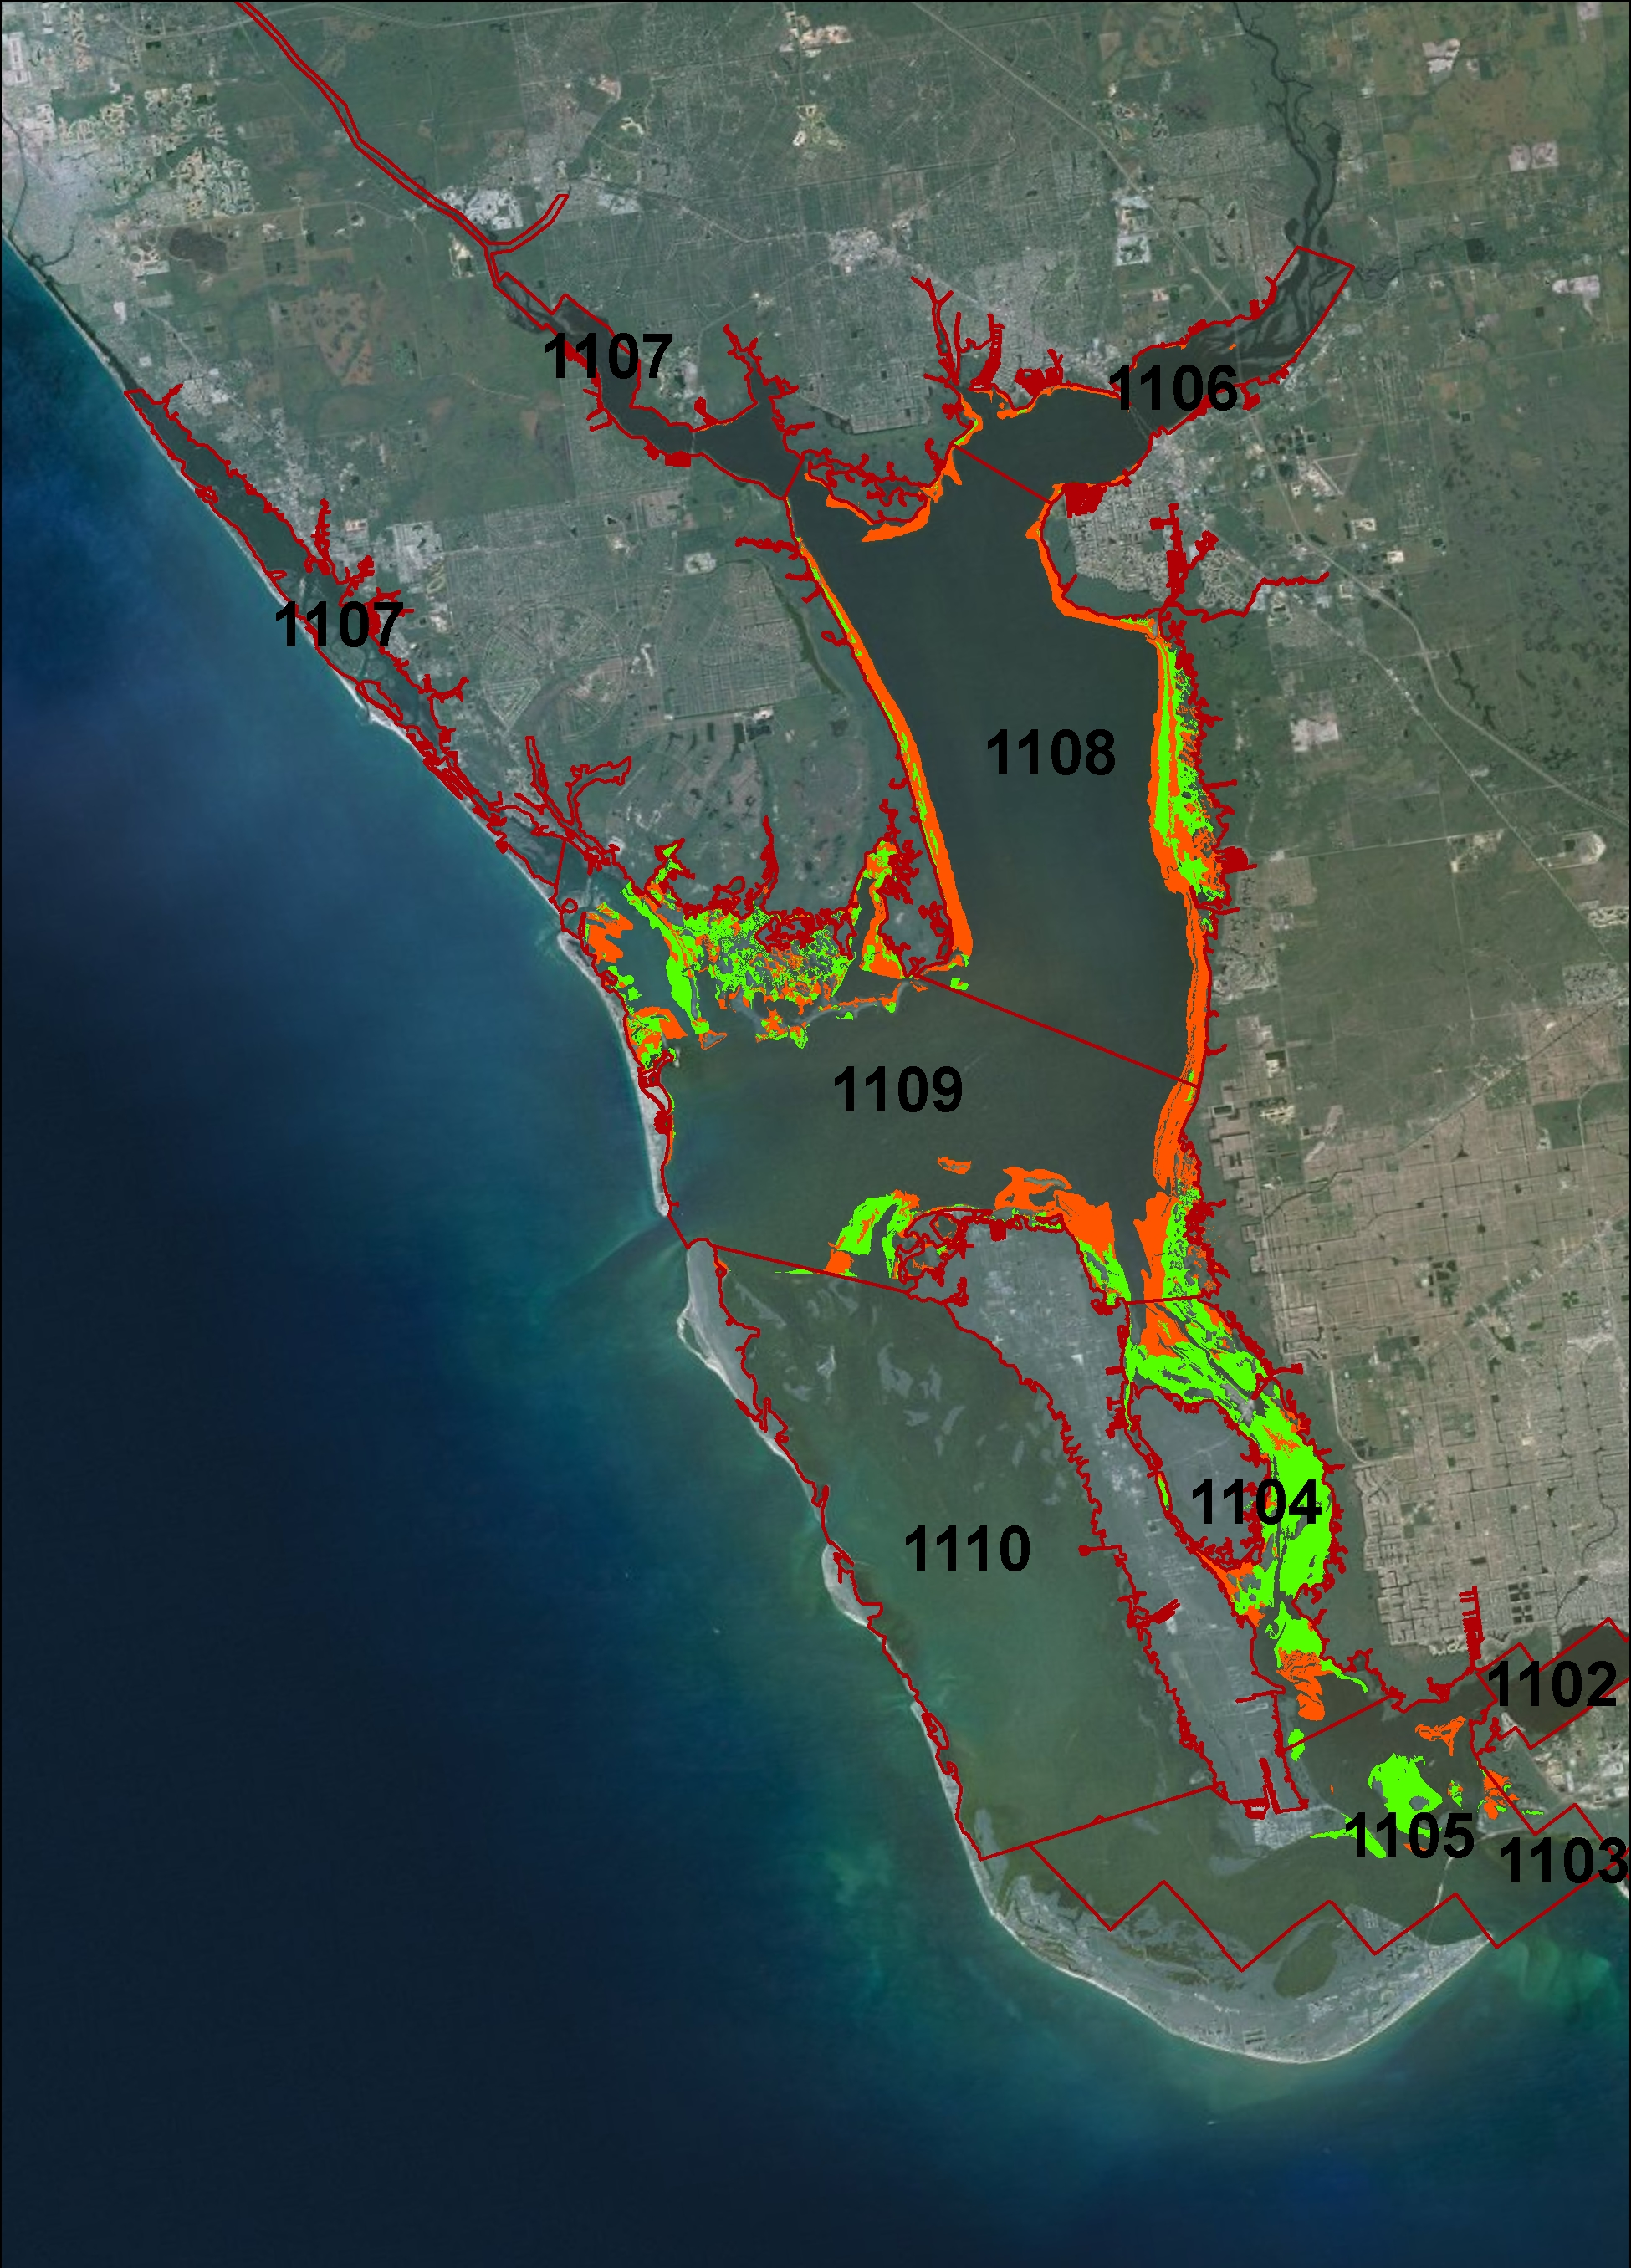
\includegraphics[width = 0.8\textwidth]{fig/Charlotte_Estuary_Segments.jpg}}
\end{column}
\end{columns}
\end{frame}

%%%%%%
\begin{frame}{\textbf{Case 2: Seagrass and water quality}}{\textbf{Making the most of existing data}}
\onslide<+->
How can we estimate depth of colonization? \\~\\
\begin{columns}[T]
\onslide<+->
\begin{column}{0.32\textwidth}
Pick a segment\\~\\
\centerline{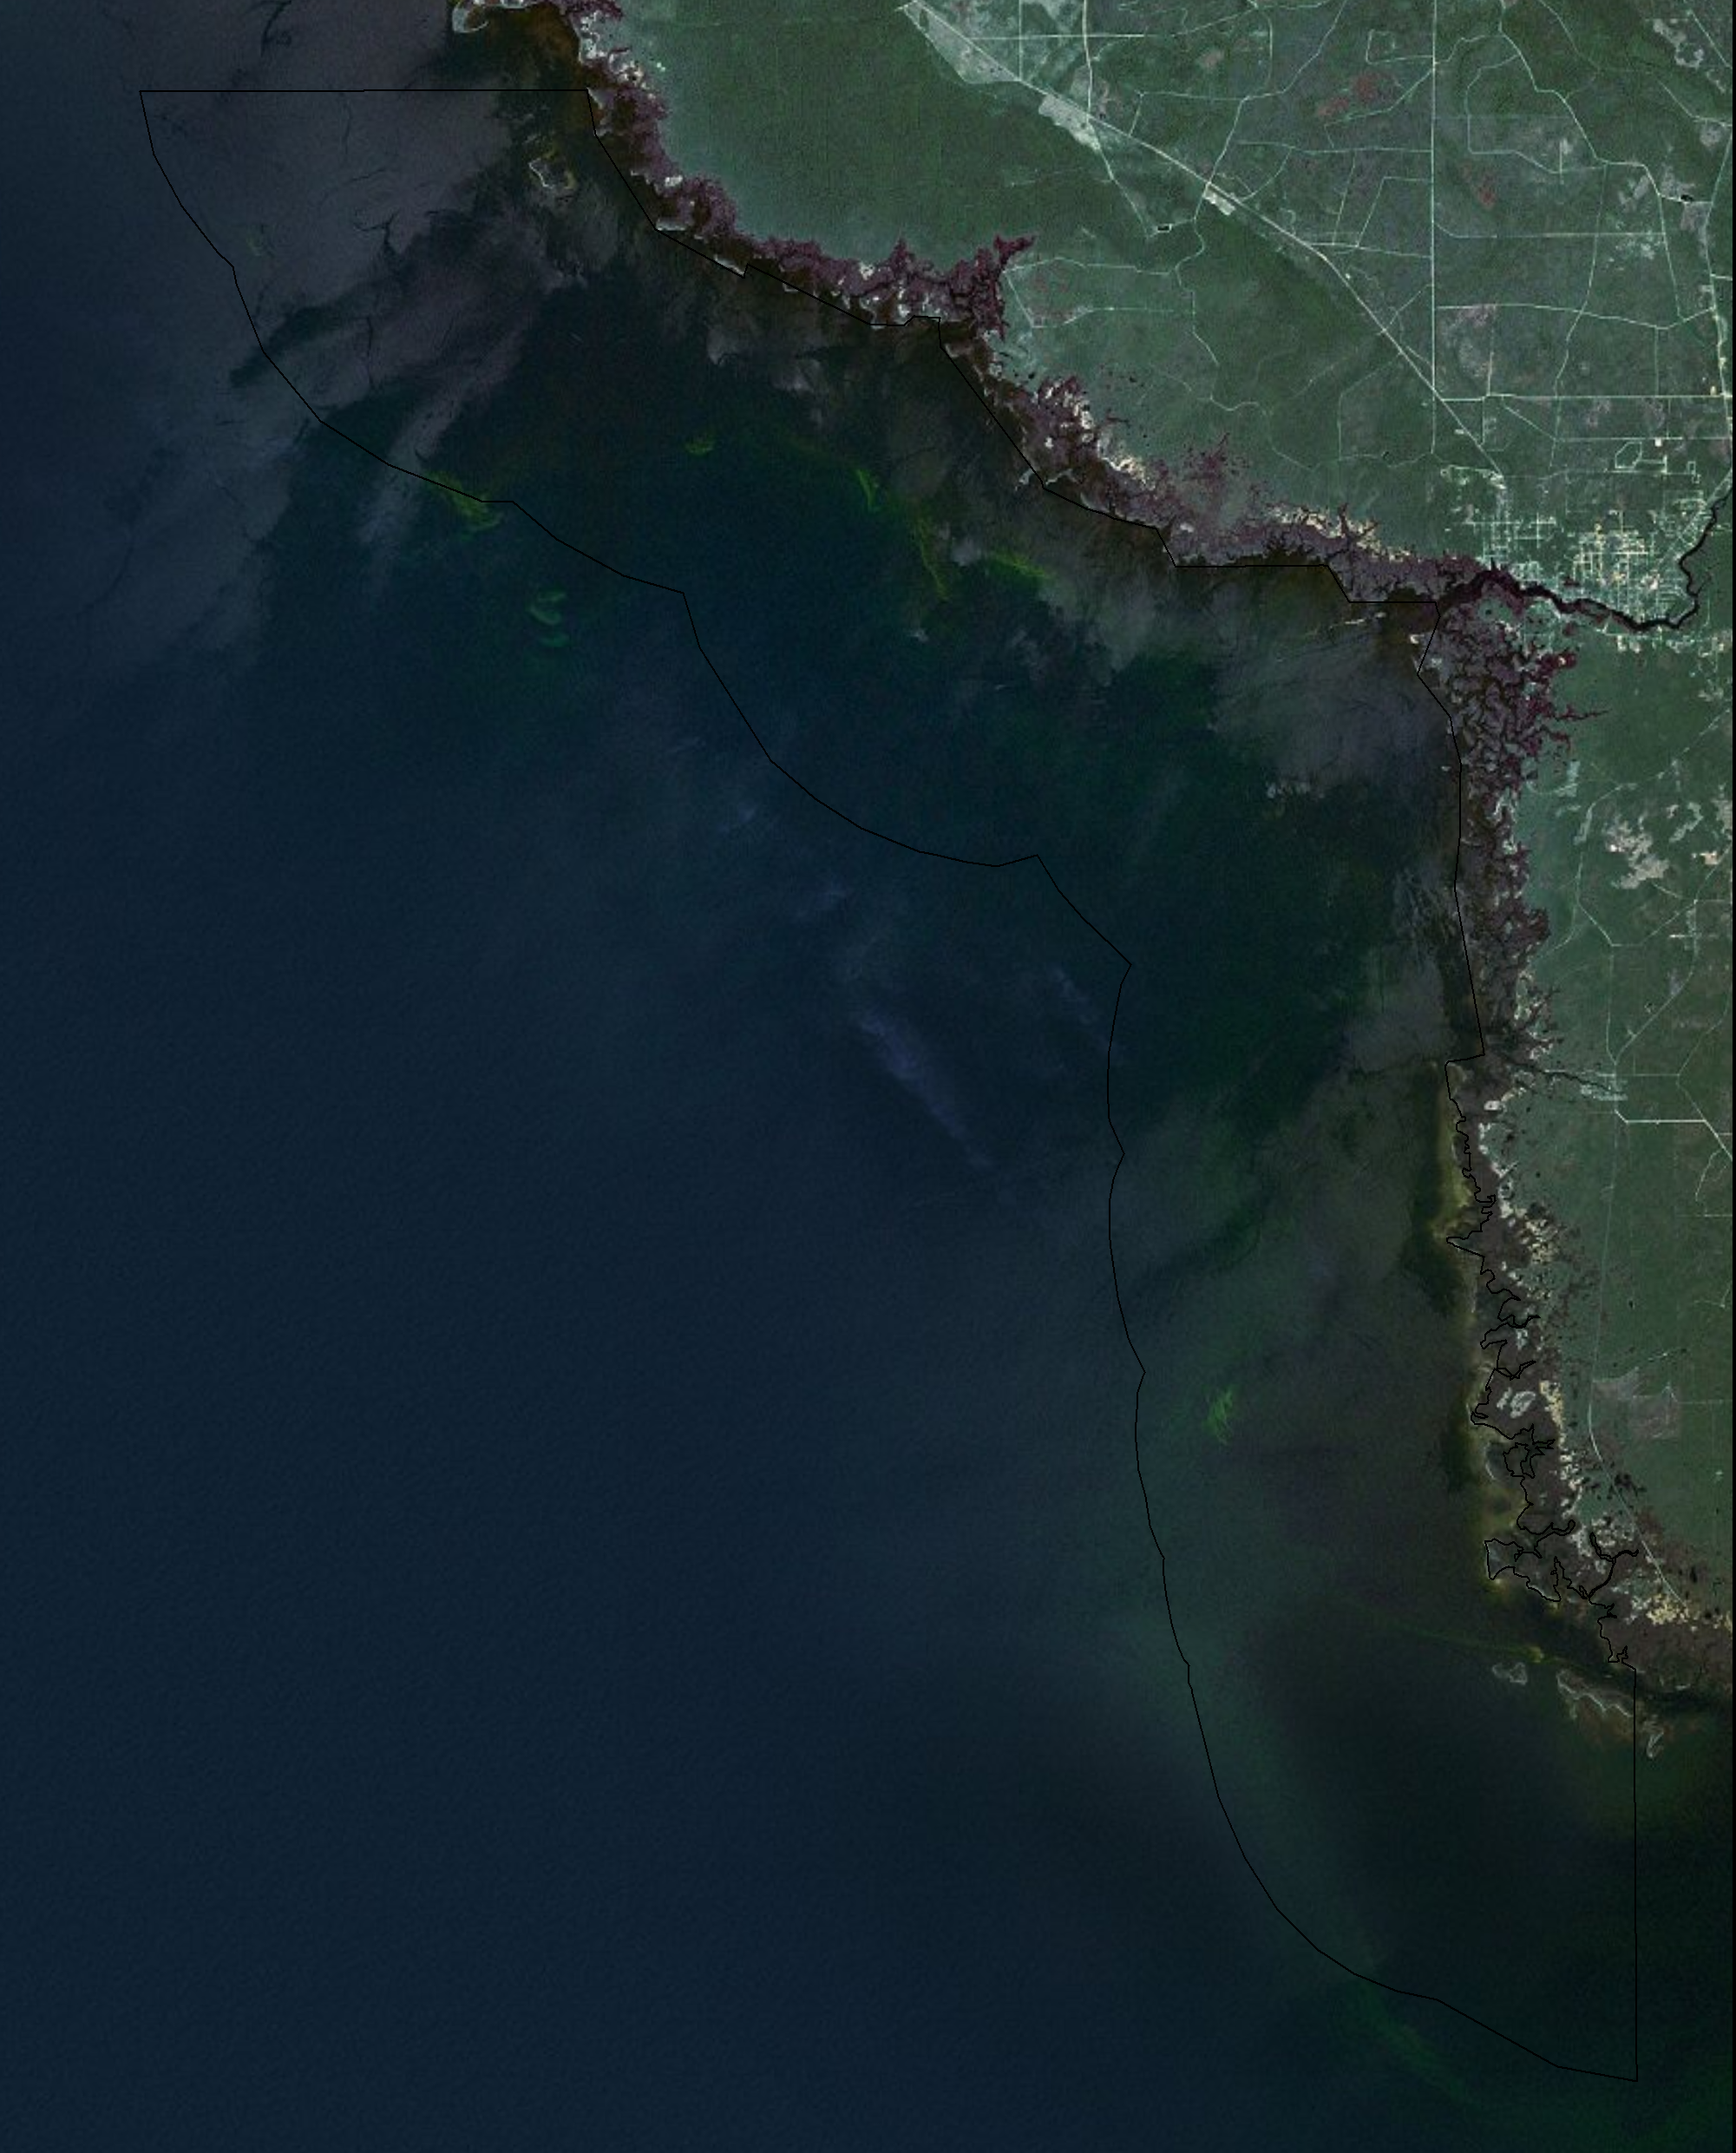
\includegraphics[width = 0.9\textwidth]{fig/map820.png}}
\end{column}
\onslide<+->
\begin{column}{0.32\textwidth}
Get seagrass coverage
\begin{knitrout}
\definecolor{shadecolor}{rgb}{0.969, 0.969, 0.969}\color{fgcolor}

{\centering 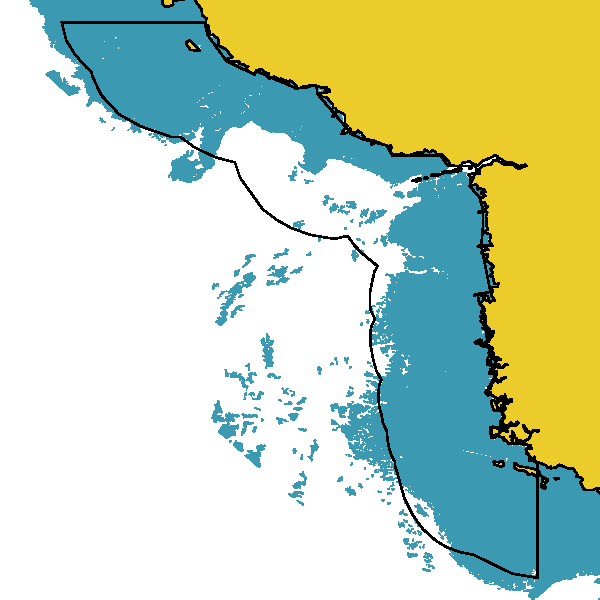
\includegraphics[width=\maxwidth]{fig//segsg} 

}



\end{knitrout}
\end{column}
\onslide<+->
\begin{column}{0.32\textwidth}
Get depth points\\~\\
\begin{knitrout}
\definecolor{shadecolor}{rgb}{0.969, 0.969, 0.969}\color{fgcolor}

{\centering 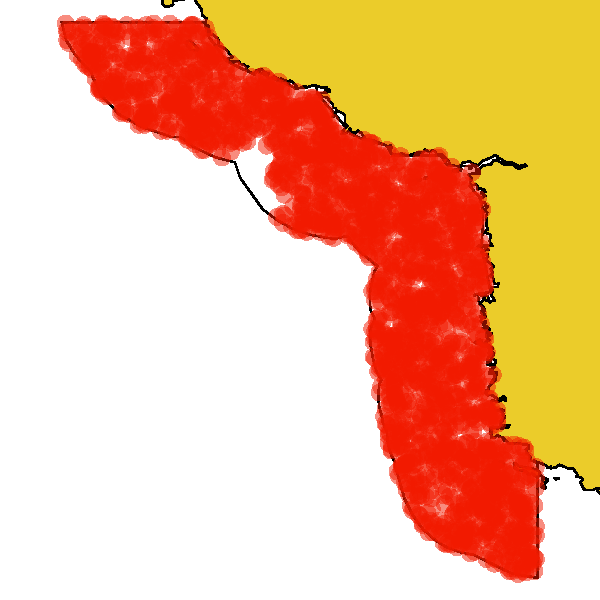
\includegraphics[width=\maxwidth]{fig//segpt} 

}



\end{knitrout}
\end{column}
\end{columns}
\end{frame}

%%%%%%
\begin{frame}{\textbf{Case 2: Seagrass and water quality}}{\textbf{Making the most of existing data}}
Plot the distribution of seagrass by increasing depth\\~\\
\centerline{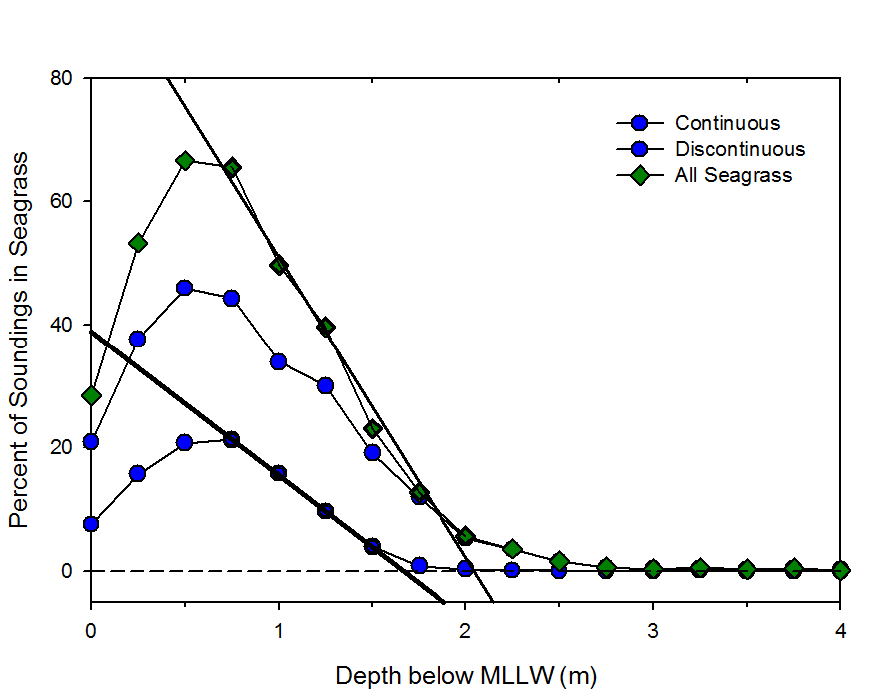
\includegraphics[width = 0.65\textwidth]{fig/Hagy_est.png}}
\vfill
\tiny
\hfill Credit: [Hagy et al., in prep]
\end{frame}



%%%%%%
\begin{frame}{\textbf{Case 2: Seagrass and water quality}}{\textbf{Making the most of existing data}}
We can get an estimate of seagrass depth of colonization for each segment in Florida \scriptsize [Hagy et al., in prep]
\vspace{-0.25in}
\centerline{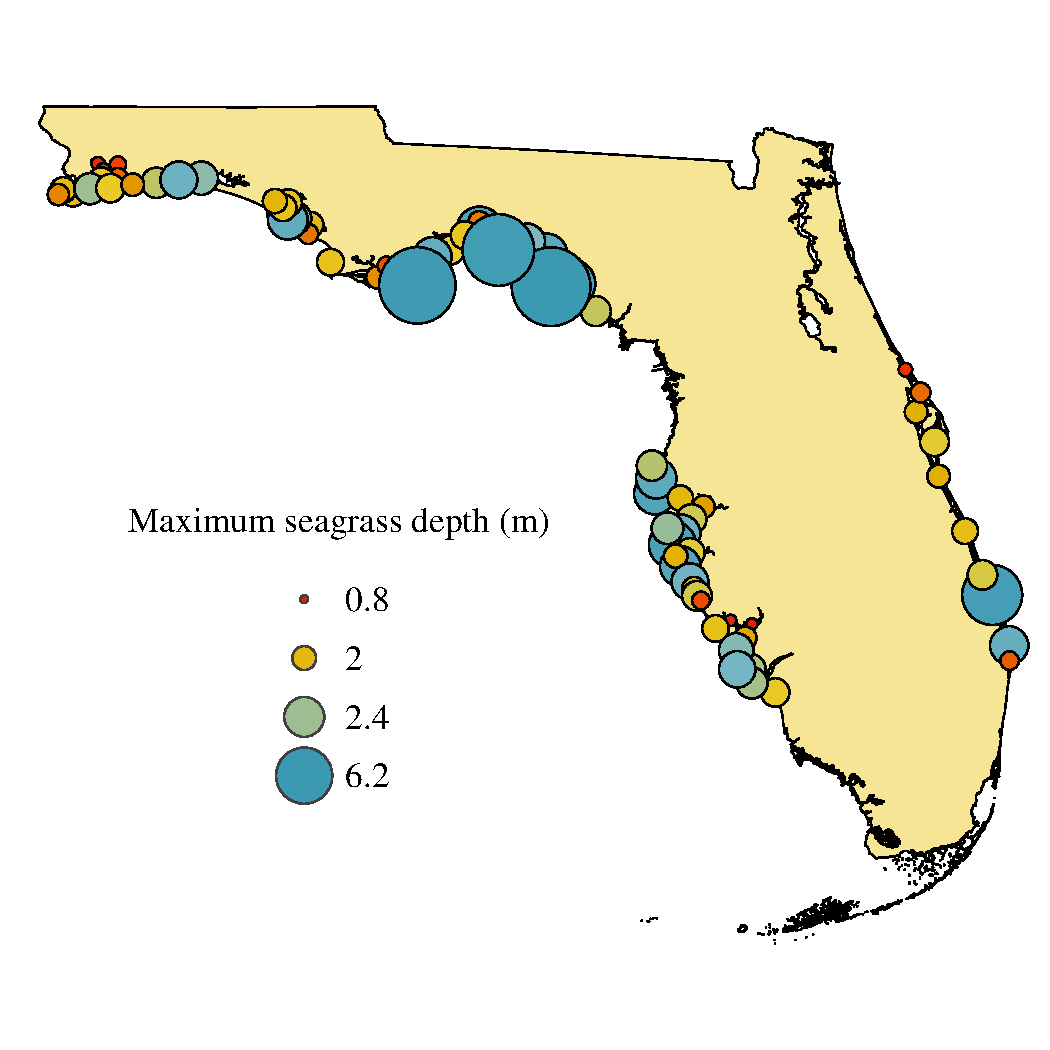
\includegraphics[width = 0.55\textwidth]{fig/sgdepthall.pdf}}
\end{frame}

%%%%%%
\begin{frame}{\textbf{Case 2: Seagrass and water quality}}{\textbf{Making the most of existing data}}
\onslide<+->
This approach works if the segment is an appropriate spatial unit to characterize seagrass...
\begin{columns}[T]
\onslide<+->
\begin{column}{0.45\textwidth}
\begin{knitrout}
\definecolor{shadecolor}{rgb}{0.969, 0.969, 0.969}\color{fgcolor}

{\centering 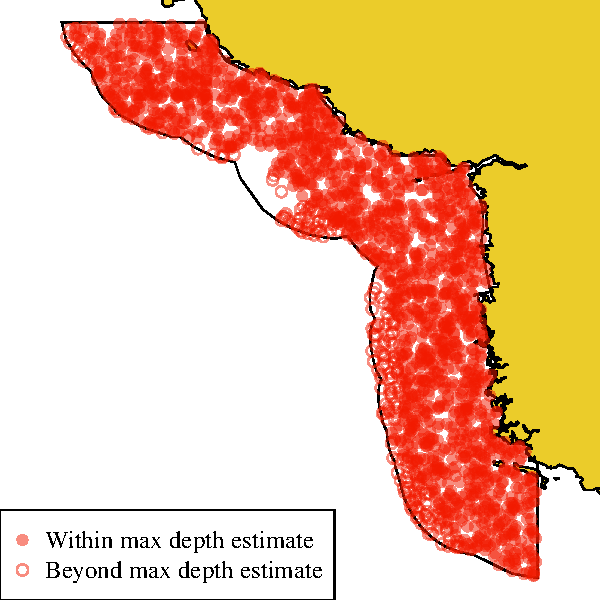
\includegraphics[width=\maxwidth]{fig//docfail1} 

}



\end{knitrout}
\end{column}
\onslide<+->
\begin{column}{0.45\textwidth}
\begin{knitrout}
\definecolor{shadecolor}{rgb}{0.969, 0.969, 0.969}\color{fgcolor}

{\centering 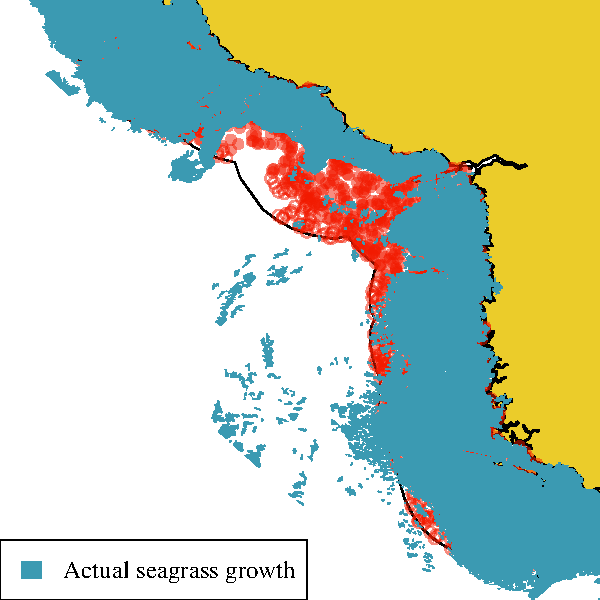
\includegraphics[width=\maxwidth]{fig//docfail2} 

}



\end{knitrout}
\end{column}
\end{columns}
\end{frame}


%%%%%%
\begin{frame}{\textbf{Case 2: Seagrass and water quality}}{\textbf{Making the most of existing data}}
If segment is not appropriate, can we define a spatial boundary for estimating seagrass depth of colonization?
\begin{center}
\animategraphics[controls,width=0.95\linewidth]{12}{fig/radred}{}{} %frame rate is 12 per/sec
\end{center}
\end{frame}


%%%%%%
\begin{frame}{\textbf{Case 2: Seagrass and water quality}}{\textbf{Making the most of existing data}}
This can be repeated for a number of points until we get estimates that make sense
\begin{center}
\animategraphics[controls,width=0.95\linewidth]{12}{fig/radred2}{}{} %frame rate is 12 per/sec
\end{center}
\end{frame}

%%%%%%
\begin{frame}{\textbf{Case 2: Seagrass and water quality}}{\textbf{Making the most of existing data}}
\onslide<+->
Benefits of the approach: \\~\\
\begin{itemize}
\item The spatial unit for any estimate of seagrass growth limit is problem-specific \\~\\
\item Allows for a `compliance-point' approach (saves time/money) \\~\\
\item Increased understanding of seagrass growth patterns - natural and anthropogenic drivers \\~\\
\end{itemize}
\onslide<+->
Lots to be done...
\end{frame}

%%%%%%
\begin{frame}{\textbf{Case 2: Seagrass and water quality}}{\textbf{Making the most of existing data}}
Development widget online: \href{https://beckmw.shinyapps.io/sg_depth/}{https://beckmw.shinyapps.io/sg\_depth/}
\centerline{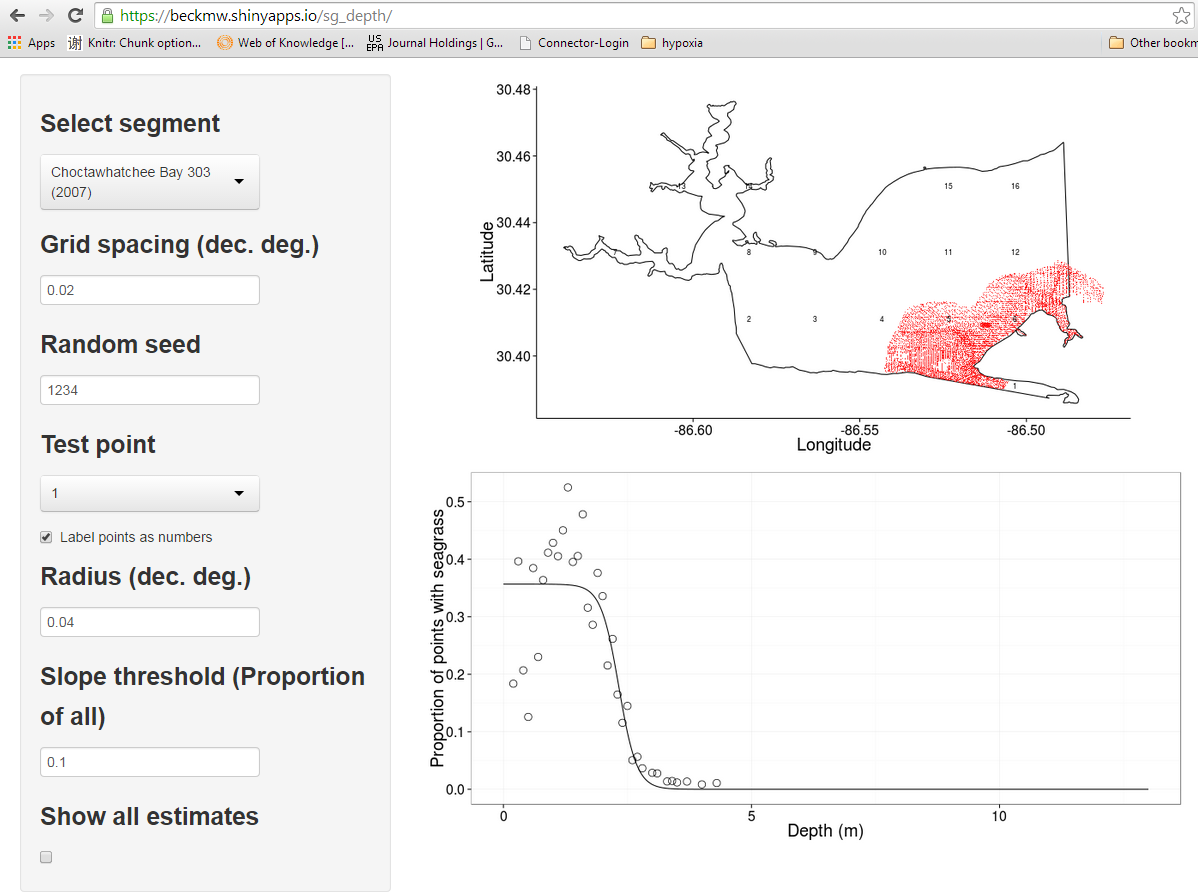
\includegraphics[width = 0.75\textwidth]{fig/widget.png}}
\end{frame}

\section{Case 3: Open-source tools}
%%%%%%
\begin{frame}{\textbf{Case 3: Open-source science}}{\textbf{Analysis tools for water quality data}}
\onslide<+->
Progress in science is incremental and builds on past work\\~\\
This requires accurate reproduction of methods\\~\\
The ability to reproduce methods will always be a challenge...\\~\\
\onslide<+->
...digital tools have proliferated to \alert{facilitate sharing}\\~\\
\begin{columns}
\begin{column}{0.25\textwidth}
\centerline{
\includegraphics[width = \textwidth]{fig/Rlogo.png}}
\end{column}
\begin{column}{0.25\textwidth}
\centerline{
\includegraphics[width = \textwidth]{fig/RStudio.png}}
\end{column}
\begin{column}{0.25\textwidth}
\centerline{
\includegraphics[width = \textwidth]{fig/knit-logo.png}}
\end{column}
\begin{column}{0.25\textwidth}
\centerline{
\includegraphics[width = \textwidth]{fig/octocat.png}}
\end{column}
\end{columns}
\end{frame}

%%%%%%
\begin{frame}{\textbf{Case 3: Open-source science}}{\textbf{Analysis tools for water quality data}}
Returning back to the System Wide Monitoring Program...\\~\\
\centerline{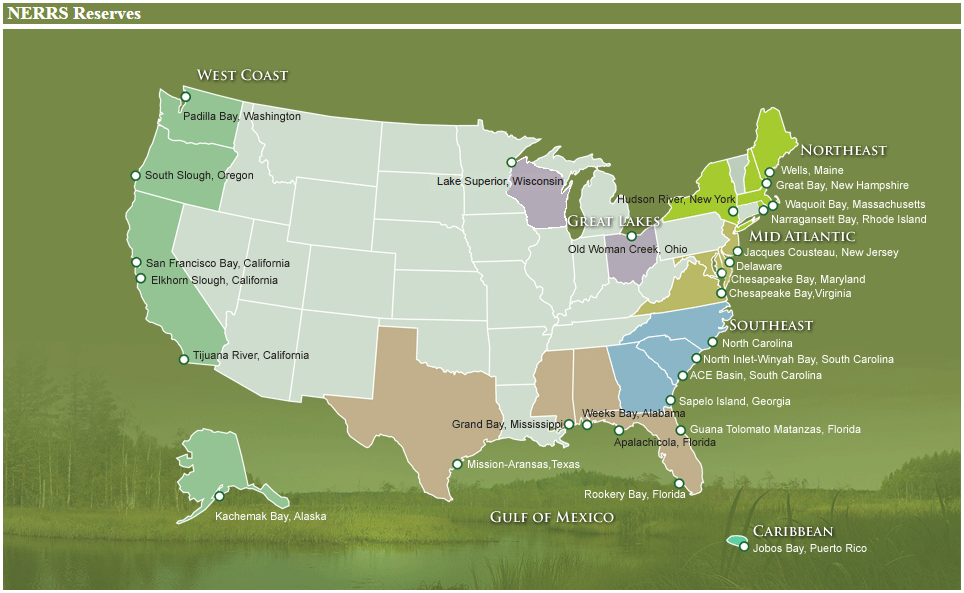
\includegraphics[width = 0.8\textwidth]{fig/NERRS_locations.png}}
\end{frame}

%%%%%%
\begin{frame}{\textbf{Case 3: Open-source science}}{\textbf{Analysis tools for water quality data}}
\onslide<+->
The SWMP database and others like it represent incredible opportunities to further our knowledge of natural systems...\\~\\
...including the effects of eutrophication \\~\\
\onslide<+->
\alert{Problem:} These data are numerous and not easily compared\\~\\
\alert{Solution:} Develop open-source tools that address the challenges of large-scale comparative analyses with continuous monitoring data\\~\\
\onslide<+->
The benefits include:
\begin{itemize}
\item Free for use by anyone
\item Free to collaborate
\item Facilitation of analysis with `under-the-hood' functionality
\end{itemize}
\end{frame}

%%%%%%
\begin{frame}{\textbf{Case 3: Open-source science}}{\textbf{Analysis tools for water quality data}}
\alert{SWMPr} is a freely available package for use with R \\~\\
Designed to facilitate the analysis of SWMP data by providing functions that...\\~\\
\begin{itemize}
\item \alert{Retrieve} SWMP data for any site and date combination \\~\\ 
\item \alert{Organize} the data using standard pre-processing techniques \\~\\
\item \alert{Analyze} the data using a suite of exploratory and graphical analysis tools \\~\\
\end{itemize}
\end{frame}

%%%%%%
\begin{frame}{\textbf{Case 3: Open-source science}}{\textbf{Analysis tools for water quality data}}
What we've done so far... estimates of ecosystem metabolism 


{\centering 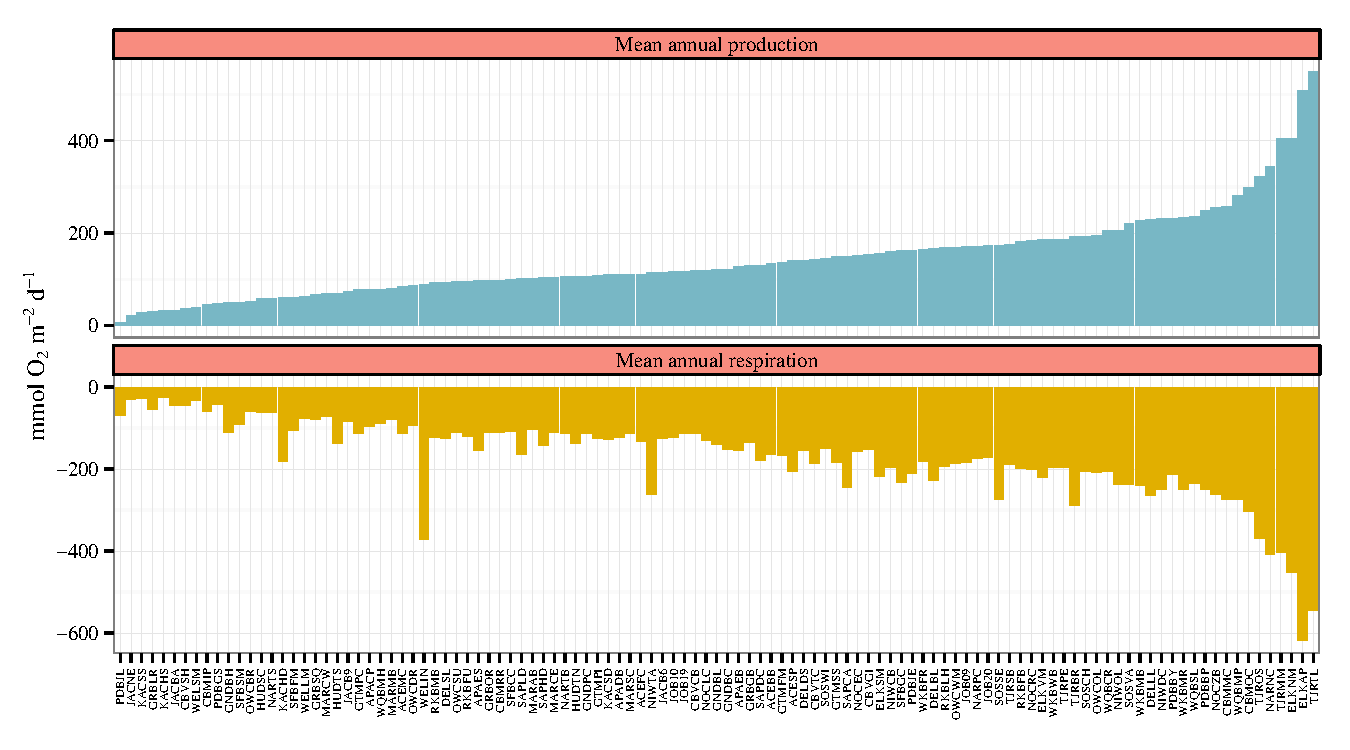
\includegraphics[width=\maxwidth]{fig//metab} 

}



\end{frame}

%%%%%%
\begin{frame}{\textbf{Case 3: Open-source science}}{\textbf{Analysis tools for water quality data}}
\onslide<+->
What we've done so far... detiding dissolved oxygen data


{\centering 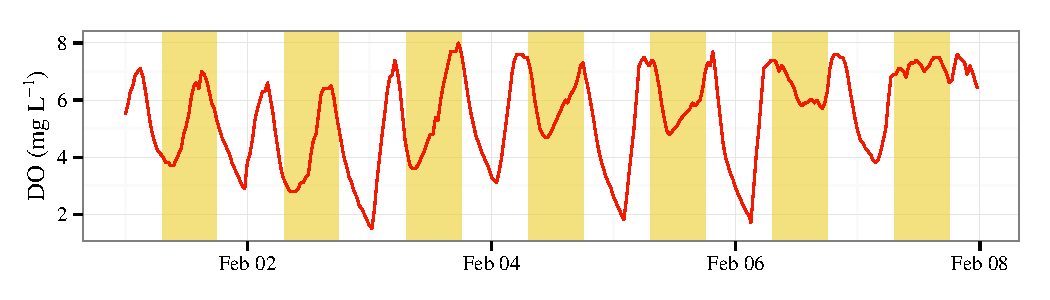
\includegraphics[width=0.9\textwidth]{fig/sapdo} 

}



\onslide<+->


{\centering 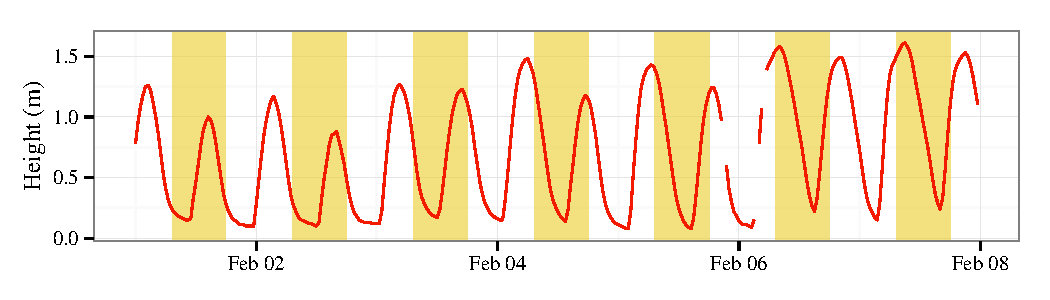
\includegraphics[width=0.9\textwidth]{fig/saptide} 

}



\end{frame}

%%%%%%
\begin{frame}{\textbf{Case 3: Open-source science}}{\textbf{Analysis tools for water quality data}}
\vspace{-0.1in}
\begin{knitrout}
\definecolor{shadecolor}{rgb}{0.969, 0.969, 0.969}\color{fgcolor}

{\centering 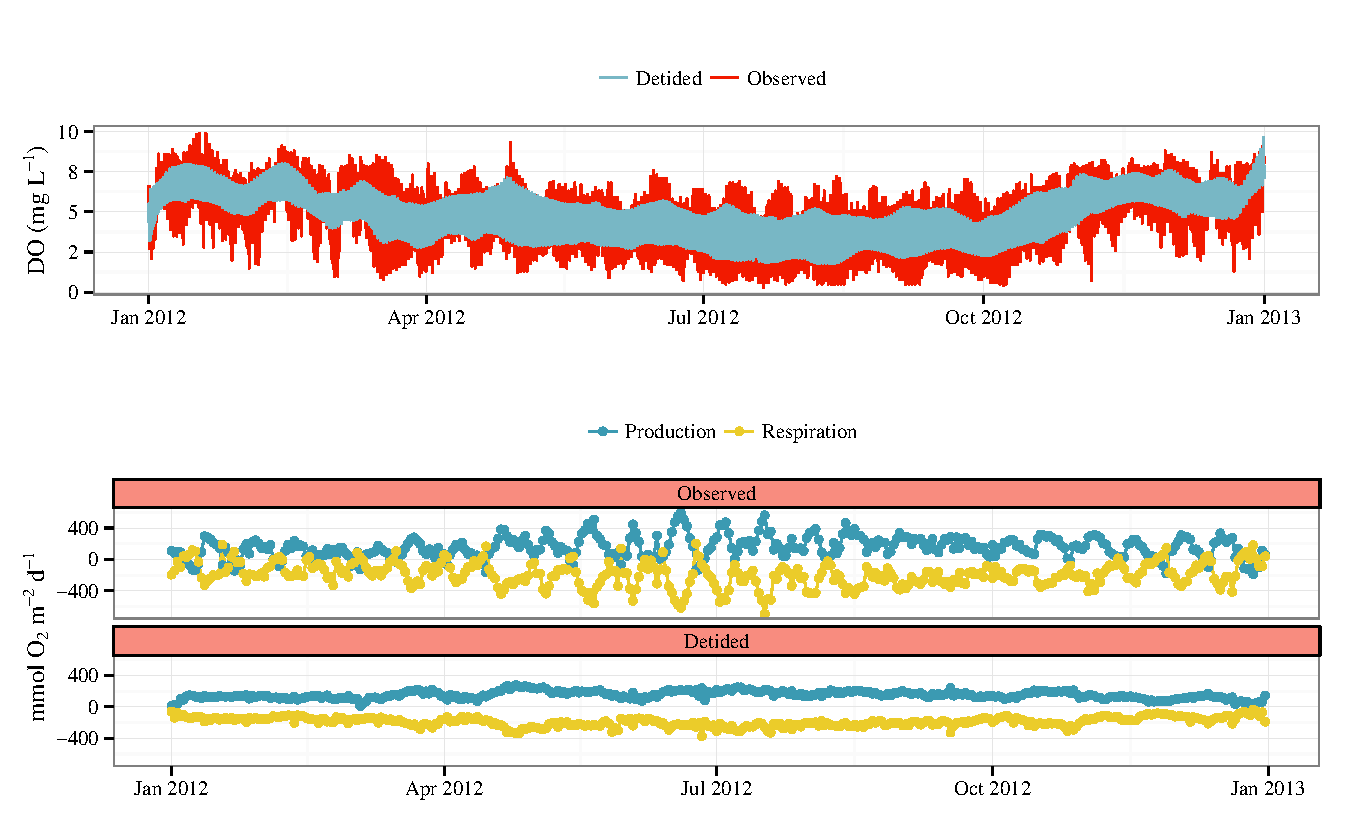
\includegraphics[width=\textwidth]{fig/dtd_met} 

}



\end{knitrout}
\end{frame}

%%%%%%
\begin{frame}{\textbf{Case 3: Open-source science}}{\textbf{Analysis tools for water quality data}}
\onslide<+->
Tools in the SWMPr package (or that will be included) have facilitated comparative analyses of millions of water quality records from NERRS \\~\\
These tools can help improve our understanding of nutrient pollution and eutrophication \\~\\
\onslide<+->
Potential for many other applications... actively being developed \\~\\
\begin{columns}
\begin{column}{0.25\textwidth}
\centerline{
\includegraphics[width = \textwidth]{fig/Rlogo.png}}
\end{column}
\begin{column}{0.25\textwidth}
\centerline{
\includegraphics[width = \textwidth]{fig/RStudio.png}}
\end{column}
\begin{column}{0.25\textwidth}
\centerline{
\includegraphics[width = \textwidth]{fig/knit-logo.png}}
\end{column}
\begin{column}{0.25\textwidth}
\centerline{
\includegraphics[width = \textwidth]{fig/octocat.png}}
\end{column}
\end{columns}
\end{frame}

\section{Conclusions}
%%%%%%
\begin{frame}{\textbf{Conclusions}}
The analysis of water quality will continue to require the use of novel tecniques to interpret the data \\~\\
These needs are motivated by: \\~\\
\begin{itemize}
\item The continued relevance of stressors that influence ecosystem conditions \\~\\
\item Our increasing ability to gather raw, uninterpreted data \\~\\
\end{itemize}
Our methods must be able to make sense of \alert{historical trends}, as well as predict \alert{future conditions}
\end{frame}

%%%%%%
\begin{frame}{\textbf{Conclusions}}
Our ability to \alert{share}, \alert{reproduce}, and \alert{collaborate} is essential \\~\\
\alert{SWMPr package:} \href{https://github.com/fawda123/SWMPr}{https://github.com/fawda123/SWMPr} \\~\\
\alert{Seagrass applications:} \href{https://beckmw.shinyapps.io/sg_depth}{https://beckmw.shinyapps.io/sg\_depth} \\~\\
\alert{Ecosystem metabolism and detiding:} \href{http://spark.rstudio.com/beckmw/detiding_cases/}{http://spark.rstudio.com/beckmw/detiding\_cases/} \\~\\
\alert{This presentation:} \href{https://github.com/fawda123/wqtrends_pres}{https://github.com/fawda123/wqtrends\_pres}
\end{frame}

%%%%%%
\begin{frame}
Acknowledgments:\\~\\
\begin{columns}
\begin{column}{0.6\textwidth}
{\footnotesize
Research staff and employees at USEPA Gulf Ecology Division - especially J. Hagy, M. Murrell\\~\\
Field staff and data managers at Hillsborough County Environmental Protection Commission\\~\\
Research coordinators of the National Estuarine Research Reserve System}\\~\\
\end{column}
\begin{column}{0.3\textwidth}
\vspace{-0.2in}
\begin{center}
{\tiny
Wes Anderson Zissou color theme borrowed and adapted from \href{https://github.com/karthik/wesanderson}{github.com/karthik}\\~\\
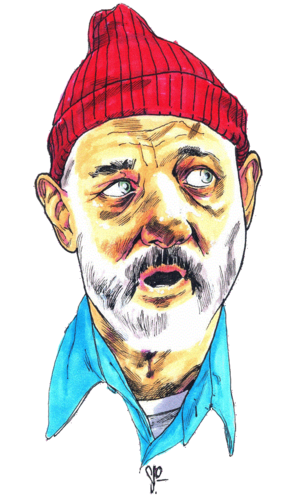
\includegraphics[width=0.55\linewidth]{fig/zissou.png}\\~\\
\vspace{-0.15in}
\scalebox{0.7}{\hbox{\tiny Image credit:\thinspace{\tiny \href{http://stephenmorrow.deviantart.com/}{Stephen Morrow}}}}}
\end{center}
\end{column}
\end{columns}
\vfill
Funding sources and contact:\\~\\
\begin{columns}
\begin{column}{0.5\textwidth}
\centerline{
\includegraphics[width=0.4\linewidth]{fig/epa_logo.png}}
\end{column}
\begin{column}{0.5\textwidth}
\scriptsize
\href{mailto:beck.marcus@epa.gov}{beck.marcus@epa.gov} \\~\\
Phone: 8509342480 \\~\\
Github: \href{https://github.com/fawda123/}{github.com/fawda123/} \\~\\
Blog: \href{http://beckmw.wordpress.com/}{beckmw.wordpress.com/}
\end{column}
\end{columns}
\vspace{0.2in}
\end{frame}

%%%%%%
\section{References}
\begin{frame}[allowframebreaks,t]{\textbf{References}}
\tiny
\setbeamertemplate{bibliography item}{}
\bibliographystyle{apalike_mine}
\bibliography{ref_diss}
\end{frame}

\end{document}
